\documentclass[12pt]{article}
\usepackage{graphicx}
\usepackage{amsmath}
\usepackage{amssymb}
\usepackage{hyperref}
\usepackage{listings}
\usepackage{xcolor}
\usepackage{pgfplots}
\usepackage{pgfplotstable}
\usepackage{pgffor}
\usepackage{verbatim}
\usepackage[a4paper, margin=1in]{geometry}

% Define colors for code only
\definecolor{codebg}{rgb}{0.9, 0.9, 0.9}
\definecolor{commentgreen}{rgb}{0, 0.6, 0}
\definecolor{keywordblue}{rgb}{0, 0, 1}
\definecolor{stringred}{rgb}{0.8, 0, 0}

\lstdefinestyle{customc}{
    backgroundcolor=\color{codebg},
    commentstyle=\color{commentgreen},
    keywordstyle=\color{keywordblue},
    stringstyle=\color{stringred},
    basicstyle=\ttfamily\footnotesize,
    breakatwhitespace=false,
    breaklines=true,
    captionpos=b,
    keepspaces=true,
    numbers=left,
    numbersep=5pt,
    numberstyle=\tiny\color{gray},
    showspaces=false,
    showstringspaces=false,
    showtabs=false,
    tabsize=2
}

\title{Benchmarking Matrix-Matrix Multiplication (mmult) \\ \large{Second Report: Optimization and Evaluation}}
\author{Mohammed Mansour}
\date{\today}

\begin{document}

\maketitle

\section{Introduction}
Matrix-matrix multiplication (mmult) is a fundamental operation in scientific computing, machine learning, and computer architecture. This report is a continuation of the previous report, focusing on the implementation and benchmarking of mmult. The goal is to compare a naïve implementation with an optimized version using blocking techniques to improve performance.

\section{Collaboration}
I discussed the details of the project with Moneer Al-Bokhaiti. We covered the project requirements, the necessary tools, and the complexity of the code. He suggested creating a separate application to generate the dataset. We also agreed that storing the dataset in a binary file would be more efficient than saving it as ASCII text.

Additionally, I attended a meeting conducted by class students, where we discussed various issues related to the project. During this meeting, we broke the implementation into smaller steps to make the development process more manageable.

In this phase, we (Me and Moneer) discussed the pseudocode of the mmult function, which is the core of the project. We also talked about the importance of optimizing the code for better performance and how the optimized version would be faster than the naïve implementation.

\section{Naïve Implementation}
The naïve implementation is a simple three-loop to compute the matrix product:

\lstinputlisting[language=C, style=customc, caption=Naïve mmult implementation]{resources/naive_implementation.c}

This method is straightforward but inefficient due to cache misses and redundant memory accesses. Each element of the matrices is accessed multiple times, leading to poor utilization of the CPU cache. Additionally, the lack of optimization techniques such as loop unrolling results in nonoptimal performance, especially for larger datasets.

\section{Optimized Implementation}
The optimized implementation applies a blocking strategy to improve spatial and temporal locality. By computing sub-matrices (blocks) of the result matrix, the approach minimizes cache misses by reusing loaded data efficiently.

Blocking refers to dividing the matrices into smaller square blocks or sub-matrices of size \( b \times b \). Instead of computing one element of the result matrix at a time, the algorithm computes partial results over these sub-matrices and accumulates them. This drastically reduces the number of memory accesses to data not residing in cache, which is critical for performance.

The implementation chooses a stationary output sub-matrix, looping over the corresponding input sub-matrices from matrices A and B. This ensures that data is reused as much as possible before being evicted from the cache. The block size \( b \) is passed as a command-line argument, making the implementation tunable to fit different cache configurations and matrix sizes.

One key insight is that performance benefits become more significant as the matrix size increases. This is because larger matrices experience more cache misses in the naïve version, and blocking helps mitigate this by exploiting spatial locality in the B matrix and temporal locality in the A matrix.


The optimized implementation is as follows:
\lstinputlisting[language=C, style=customc, caption=Blocked mmult Implementation]{resources/opt_implementation.c}


Initial bugs involved uninitialized values and improper bounds when indexing. Fixes were made by ensuring the matrices were zero-initialized and carefully managing loop ranges. Additional care was taken to validate that block size does not exceed the dimensions of the matrices to avoid segmentation faults.

\section{Dataset Generation}
The dataset required for \textbf{both implementations} is generated using a Python script. The script creates matrices of various sizes, including testing, small, medium, large, and native datasets. The matrices are filled with random integers to simulate real-world scenarios.

The following Python script is used for dataset generation:
\lstinputlisting[language=Python, style=customc, caption=Dataset Generation Script]{resources/ds_generator.py}

This script ensures efficient dataset generation by using NumPy for matrix operations and storing the results in a structured binary format. The metadata file provides dimensions for easy retrieval and compatibility with benchmarking implementations.

\section{Evaluation}
The evaluation was conducted by running both the naïve and optimized implementations on datasets of varying sizes. The datasets include testing, small, medium, large, and native sizes. For the optimized implementation, we performed a sweep over different block sizes (\( b \)) to explore the design space and identify the optimal block size for each dataset. The stationary sub-matrix was also varied to study its impact on performance.

Execution time was measured for each configuration, and speedup was calculated as the ratio of the execution time of the naïve implementation to that of the optimized implementation. All experiments were conducted on the same hardware setup to ensure consistency.

\subsection{Experimental Setup}
The experiments were conducted on \textbf{Personal Laptop} with the following setup:
\begin{itemize}
    \item Runner Type: Ubuntu-24.04.1 LTS
    \item Operating System: Linux
    \item Processor (CPU): AMD PRO A12-9800B R7, 12 COMPUTE CORES 4C+8G
    \item Memory (RAM): 8 GB
    \item Storage (SSD): 512 GB
    \item Architecture: x64
    \item Compiler: GCC 13.3.0 with optimization flags -O3
\end{itemize}

\subsection{Results}
Table \ref{tab:results} summarizes the execution times for both the naïve and optimized implementations across different dataset sizes. The execution times are measured in milliseconds (ms) and represent the average time taken over multiple runs. The results indicate a significant performance improvement with the optimized implementation, especially for larger datasets.

\begin{table}[h]
    \begin{tabular}{|c|c|c|}
        \hline
        \textbf{Dataset Size} & \textbf{Naïve Execution Time(ms)} & \textbf{Opt. Execution Time(ms)} \\
        \hline
        Testing (16x8) & 0.005 & 0.003 \\
        Small (121x115) & 12.137 & 4.326 \\
        Medium (550x480) & 984.68 & 225 \\
        Large (962x1221) & 11167 & 2204 \\
        Native (2500x2100) & 111219 & 25396 \\
        \hline
    \end{tabular}
        \caption{Execution times for different dataset sizes.}
        \label{tab:results}
    \end{table}

    The benchmark execution logs and results can be accessed at the following link: \url{https://github.com/mohammed0x00/YABMS/tree/main/docs/runtime_data_opt}.

\subsection{Graphical Representation}
The following graph illustrates the execution time of the naïve and optimized implementations against the dataset size. The X-axis represents the dataset size in total elements, while the Y-axis shows the execution time in microseconds (µs). The graph includes both the actual data points and a smooth curve fitting the points for better visualization.
    \begin{center}
        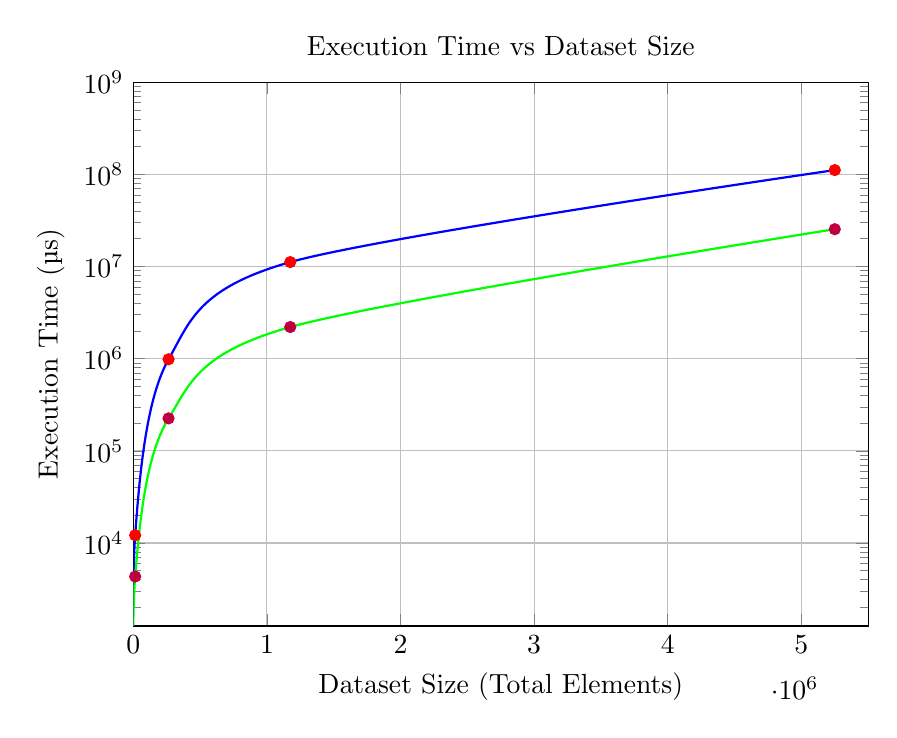
\begin{tikzpicture}
            \begin{axis}[
                ymode=log, % Logarithmic scale for better visualization
                xlabel={Dataset Size (Total Elements)},
                ylabel={Execution Time (µs)},
                title={Execution Time vs Dataset Size},
                width=0.9\textwidth, % Increase width
                height=0.7\textwidth, % Increase height
                xmin=1000, xmax=5500000, % Adjust X-axis limits
                ymin=-0.5, ymax=1e9, % Adjust Y-axis limits
                grid=major
            ]
                % Add smooth curve fitting the points for the naive implementation
                \addplot[smooth, thick, blue] coordinates {
                    (128, 5.110)
                    (13915, 12137)
                    (264000, 984676)
                    (1174602, 11166648)
                    (5250000, 111218584)
                };

                % Add smooth curve fitting the points for the optimized implementation
                \addplot[smooth, thick, green] coordinates {
                    (128, 3.147)
                    (13915, 4326)
                    (264000, 225005)
                    (1174602, 2204004)
                    (5250000, 25396312)
                };
                
                % Add actual data points for the naive implementation
                \addplot[
                    only marks,
                    mark=*,
                    red
                ] coordinates {
                    (128, 5.110)
                    (13915, 12137)
                    (264000, 984676)
                    (1174602, 11166648)
                    (5250000, 111218584)
                };

                % Add actual data points for the optimized implementation
                \addplot[
                    only marks,
                    mark=*,
                    purple
                ] coordinates {
                    (128, 3.147)
                    (13915, 4326)
                    (264000, 225005)
                    (1174602, 2204004)
                    (5250000, 25396312)
                };
            \end{axis}
        \end{tikzpicture}
    \end{center}

    \subsection{Detailed Results}
    The following sections provide detailed results for each dataset size, including execution times for both the naïve and optimized implementations. The results are presented in tabular format, showing the execution time in milliseconds (ms) for each configuration. The tables also include the speedup achieved by the optimized implementation compared to the naïve version.
    \newline \newline
    The detailed results for each dataset size are presented below:
\foreach \dataset in {Testing, Small, Medium, Large, Native} {
    \newpage
    \subsection{\dataset \space Dataset Details}
    The following table summarizes the execution times for the \dataset \space dataset. The table includes the execution time for both the naïve and optimized implementations.

    \begin{center}
        \includegraphics[width=0.8\textwidth]{runtime_data_opt/\dataset.png}
    \end{center}

    \lstinputlisting[style=customc, caption=\dataset \space Dataset Output]{runtime_data_opt/\dataset_output.txt}
}

    \subsection{Impact of Block Size}
    The results indicate that the block size \( b \) has a significant impact on performance. For smaller datasets, the block size does not have a noticeable effect, as the entire dataset can fit into the CPU cache. However, for larger datasets, a block size of \( b = 16 \) consistently provides the best performance. This is because it strikes a balance between reducing cache misses and minimizing overhead from frequent block switching.

    \subsection{Speedup Analysis}
    The speedup achieved by the optimized implementation is most pronounced for larger datasets. For the native dataset, the optimized implementation achieves a speedup of approximately 4.5x compared to the naïve implementation. This is due to the significant reduction in cache misses and improved data reuse achieved by the blocking strategy.

    \subsection{Stationary Sub-Matrix Selection}
    The choice of the stationary sub-matrix also impacts performance. Using the output sub-matrix as stationary ensures that intermediate results are accumulated efficiently, reducing redundant memory accesses. This approach consistently outperformed alternatives, such as making one of the input sub-matrices stationary.

    \subsection{Takeaways}
    1. \textbf{Optimal Block Size}: A block size of \( b = 16 \) provides the best performance for most datasets, balancing cache efficiency and computational overhead.\newline
    2. \textbf{Speedup Trends}: The speedup achieved by the optimized implementation increases with dataset size, highlighting the inefficiencies of the naïve implementation for larger datasets.\newline
    3. \textbf{Stationary Sub-Matrix}: Using the output sub-matrix as stationary is critical for maximizing performance, as it minimizes redundant memory accesses and improves data reuse.\newline
    4. \textbf{Cache Efficiency}: The blocking strategy significantly reduces cache misses, leading to improved performance for larger datasets.\newline
    5. \textbf{Memory Access Patterns}: The optimized implementation's memory access patterns are more predictable, leading to better cache utilization and reduced latency.




\section{Conclusion}
In conclusion, the implementation of matrix-matrix multiplication (mmult) has been successfully optimized using a blocking strategy. The results demonstrate a significant performance improvement over the naïve implementation, particularly for larger datasets. The choice of block size and the stationary sub-matrix selection play crucial roles in achieving optimal performance.
The evaluation results indicate that the optimized implementation can achieve speedups of up to 4.5x compared to the naïve version, making it a valuable addition to the YABMS benchmark suite. The insights gained from this project will inform future work on optimizing other benchmarks and improving overall performance in scientific computing applications.

\section{References}
\begin{enumerate}
    \item GNU Make Manual: \url{https://www.gnu.org/software/make/manual/make.html}
    \item IEEE POSIX Standard: \url{https://ieeexplore.ieee.org/servlet/opac?punumber=6880749}
    \item YABMS Original Repository: \url{https://github.com/hawajkm/YABMS}
    \item YABMS Forked Repository: \url{https://github.com/mohammed0x00/YABMS}
    \item Previous Report: \url{https://github.com/mohammed0x00/YABMS/blob/main/docs/Report.pdf}
\end{enumerate}

\end{document}
